\appendix
\section{Glossary, abbreviations and acronyms}

\begin{description}
\item[APA] Anode Plave Assembly
\item[CIS] Continuous Integration System
\item[CVMFS] CERN Virtual Machine File System (network-based method of data delivery)
\item[FS] Full Stream (data collected with zero threshold)
\item[HE] High-Energy threshold and data stream associated with it
\item[LBNF] Long-Baseline Neutrino Facility
\item[NDS] Near Detector Systems
\item[RCE] Reconfigurable Cluster Element
\item[SAM] \textit{Sequential Access via Metadata} (a metadata and storage system at FNAL)
\item[SNB] Supernova Burst
\item[SiPM] Silicon Photo-Multiplier
\item[SSP] SiPM (Silicon Photomultiplier) Signal Processor
\item[WMS] Workload Management System
\item[ZS] Zero Suppression
\end{description}

%%%%%%%%%%%%%%%%%%%%%%%%%%%
\section{Event Reconstruction for the Liquid Argon TPC}
\label{sec:reconstruction}
\subsection{Implications of Wire Readout}
Time Projection Chambers used in experiments like STAR at RHIC and ALICE at the LHC~\cite{alice}  feature
pad-based readout scheme, which allows for a relatively straightforward reconstruction of 2D patterns in
a given time slice. However, using pads in larger detectors is not practical due to power consumption considerations
(and requisite cooling requirements), excessive cost of readout electronics and other factors. For this reason, due
to its sheer size, the DUNE LArTPC features wire-based readout to cover its extremely large fiducial volume while
keeping the channel count realistic. This makes its large scale possible, but also leads to a loss of spatial information
being available for reconstruction (when compared to pads).

In order to properly describe the problem of event reconstruction in DUNE, it is helpful to explain
features and implications of the wire readout. We start with a diagram in Fig.~\ref{fig:signal-0}, the meaning of which will be detailed below.
\label{sec:wirecell}
\begin{figure}[h!]
	\centering
	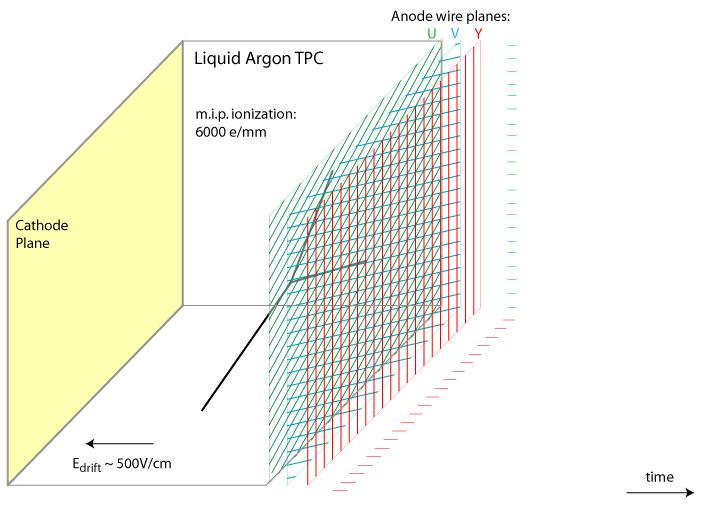
\includegraphics[width=0.9\textwidth]{signal-0.png}
	\caption{Liquid Argon TPC with wire readout: principle of operation}
	\label{fig:signal-0}
\end{figure}

The Liquid Argon Time Projection Chamber (LArTPC) is in essence a specially instrumented ionization chamber. Charges (electrons and positive ions)
created due to passage of ionizing particles through the sensitive medium (argon in this case) are subject to the effect of a uniform electrostatic
field which is created in Liquid Argon by a system of cathode and anode electrodes, which causes them to move (drift) along the field lines.
If there is an additional electrode within the Liquid Argon volume in the vicinity of the drifting charge, there will be a signal induced on it. Multiple such
electrodes (sensors) provide means for spatial characterization of the ionization charge distribution in the sensitive volume (which for example may
correspond to a particle track). Importantly, the shape of the signals on the electrode vs time is used to measure charge localization along the drift
direction (hence the term ``Time Projection Chamber''). For example, ionization electrons which are closer to the collection electrode will arrive to it sooner than
more distant ones, therefore time evolution of the signals on the affected wires will reflect distribution of the charge along the drift axis.

Current design of large scale LArTPC devices features planar arrays of wire electrodes supported by
rectangular frames. Such design contains an essential element called \textit{Anode Plane Assembly} (APA), which includes the ``collection plane'' (anode)
and two planes of sensor wires, called ``induction planes'', oriented at stereo angles with respect to each other and the collection plane.
Due to stereo angles, such arrangement allows for 2D measurement of the charge density distribution in the APA plane.
This is illustrated in Fig.~\ref{fig:signal-0}, which schematically shows the drift volume (to the left), the induction planes ``U'' and ``V'' and
the collection plane ``Y''. An important feature of such arrangement is that the \textit{same drifting charge} is measured three times as it
is detected by the three wire planes. This is further illustrated in Fig.~\ref{fig:3projections} as a schematic of drifting charge creating signals on wires,
represented conceptually as a view along the direction of the drift.

\begin{figure}[h!]
	\centering
	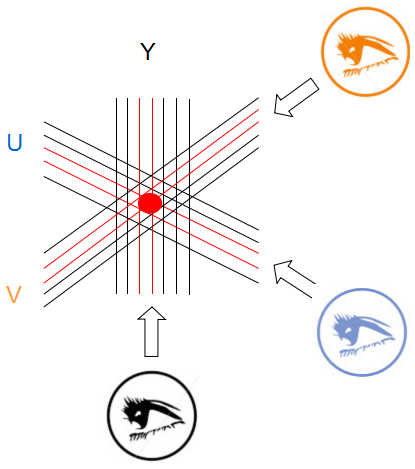
\includegraphics[width=0.65\textwidth]{uvy_2.png}
	\caption{Three projections of an object in a TPC with wire-based readout}
	\label{fig:3projections}
\end{figure}

Using just three projections to reconstruct an extended object (ionization charge density) presents challenges for event reconstruction.
Reliability and thorough characterization of the algorithms employed in this area will be critical for the systematics and other performance characteristics of DUNE.

There are a few approaches currenlty in development for event reconstruction. The ``Pandora'' toolkit (\ref{sec:wirecell}), which
originated as R\&D for fine-grained calorimetry at ILC~\cite{pandora}, is being adopted to reconstruct LArTPC events.
In addition, there is a ``projection matching algorithm'' which will be used for test-beam studies with protoDUNE detector.

There is also a promising toolkit under development (called ``Wire Cell'') based on a different approach.
It performs three-dimensional imaging of events using the principles commonly applied in tomography.
As is frequently the case in tomographic reconstruction with sparse data, this may require the use memory- and CPU-intensive computing platforms.
It is likely that meeting the demands of such calculations will require adopting emerging technologies that are now becoming more common in
HEP, such as GPU or other co-processor acceleration and/or massively parallel systems such as HPC facilities.

\subsection{Pandora}
\label{sec:pandora}
 Pandora is a toolkit for implementing pattern recognition algorithms for fine-grain detectors, based on the so-called ``particle flow'' approach~\cite{pandora}.
It was conceived as a way to improve resolution of calorimetric measurements by taking advantage of the detector granularity. Pandora incorporates a
number of algorithms for different stages of event reconstruction, such as clustering algorithm, topological association algorithms, track-cluster association
algorithms and others, while providing a framework to utilize and manage these components. The framework also deals with memory management
and is designed to minimize external dependencies.

Pandora was adopted for event reconstruction in LBNE and now continues as a DUNE effort. It has been incorporated into the LArSoft sofware toolkit
as a package.



\subsection{Wire Cell}
\label{sec:wirecell}
\subsubsection{The Inverse Problem}

The LArTPC acts an imaging device, i.e. the physics information about the processes taking place in the detector volume is extracted by
analysing the 3D structures (images) of ionization patterns produced by particles participating in these processes. The only source of information
available for reconstruction of these images are amplitudes of signals coming from the wires in (U,V,Y) recorded as a function of time
as described above. It follows that the event reconstruction problem in DUNE TPC is a fairly typical case of the \textit{Inverse Problem},
where a 3D structure must be calculated based on a set of observables.

Because of time quantization inherent in operation of ADC, the 3D image effectively becomes an assembly of 2D slices.
In a given time slice, the 2D charge density distribution is observed via three different projections along the axes (U,V,Y) (see Fig.~\ref{fig:3projections}).
There is substantial similaritiy between this type of inverse problem and Computed Tomography (CT) with limited projection data. This similarity becomes even more prominent as we observe that in a
given slice the charge signals on wires are essentially linear integrals of the 2D charge density along each of the three observation axes. Common with many tomographic applications, the reconstruction strategy
then consists of calculating patterns in each 2D slice and then combining them into a full 3D structure. There are many event types and topologies
in DUNE, one example of a simulated neutral-current event in presented in Fig.~\ref{fig:ncc-example-1}.

\begin{figure}[h!]
	\centering
	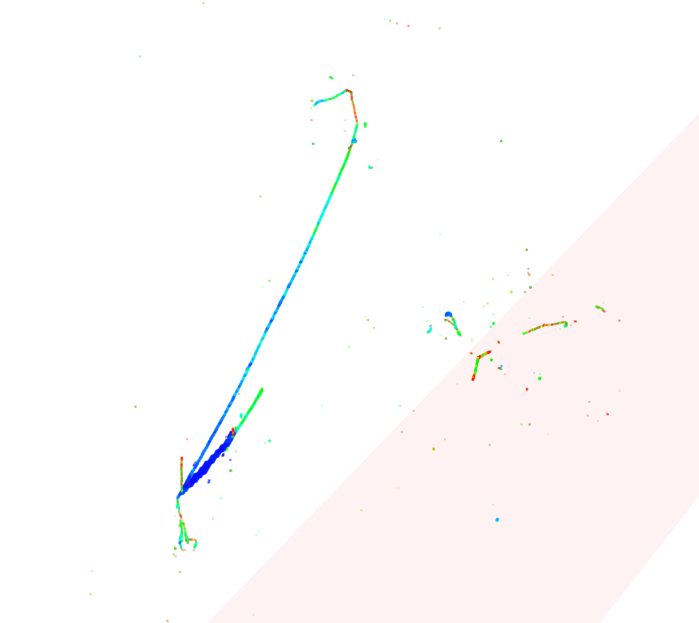
\includegraphics[width=0.7\textwidth]{ncc-example-1.png}
	\caption{An example of a neutrino-induced reaction in Liquid Argon ( simulation)}
	\label{fig:ncc-example-1}
\end{figure}

It's easy to see that (again, similar to majority of tomographic application) the reconstruction problem in DUNE is an ill-posed one,
due to the very limited set of just three observation angles. At the most basic level, this issue
manifests itself as ``ghost hits'' (well known in HEP), which is an ambiguity inherent in stereo
projection measurements.

The ``Wire Cell'' approach to this problem is based on the following:
\begin{itemize}
\item ``Voxelization'' of the TPC volume by treating each 2D slice as a tessellation (i.e. consisting of polygon-shaped tiles).

\item Solving an optimization problem which maximizes the likelihood of a given configuration of tiles (with charge associated with them) producing the observed signal distribution on the wires.

\item In reference to the optimization problem described above: regularization based on testing hypotheses about the object topology, e.g. that it's a track in a given portion of the volume. For example, cells in adjacent time slices can be tested for proximity in 2D.
\end{itemize}

To make this approach possible, there is one prerequisite that must be met, and that is a precise measurement of charge on each wire. This involves
proper calibration of the detector as well as solution of yet another inverse problem -- deconvolution of the detector and electronics reponse while
reconstructing the original shape of the charge signal. This is done in conditions of non-zero noise and involves applicaiton of digital filtering techniques.

\subsubsection{Wire Cell Components}
The flow of data in Wire Cell is presented in Fig.~\ref{fig:wirecell-diagram}.
\begin{figure}[h!]
	\centering
	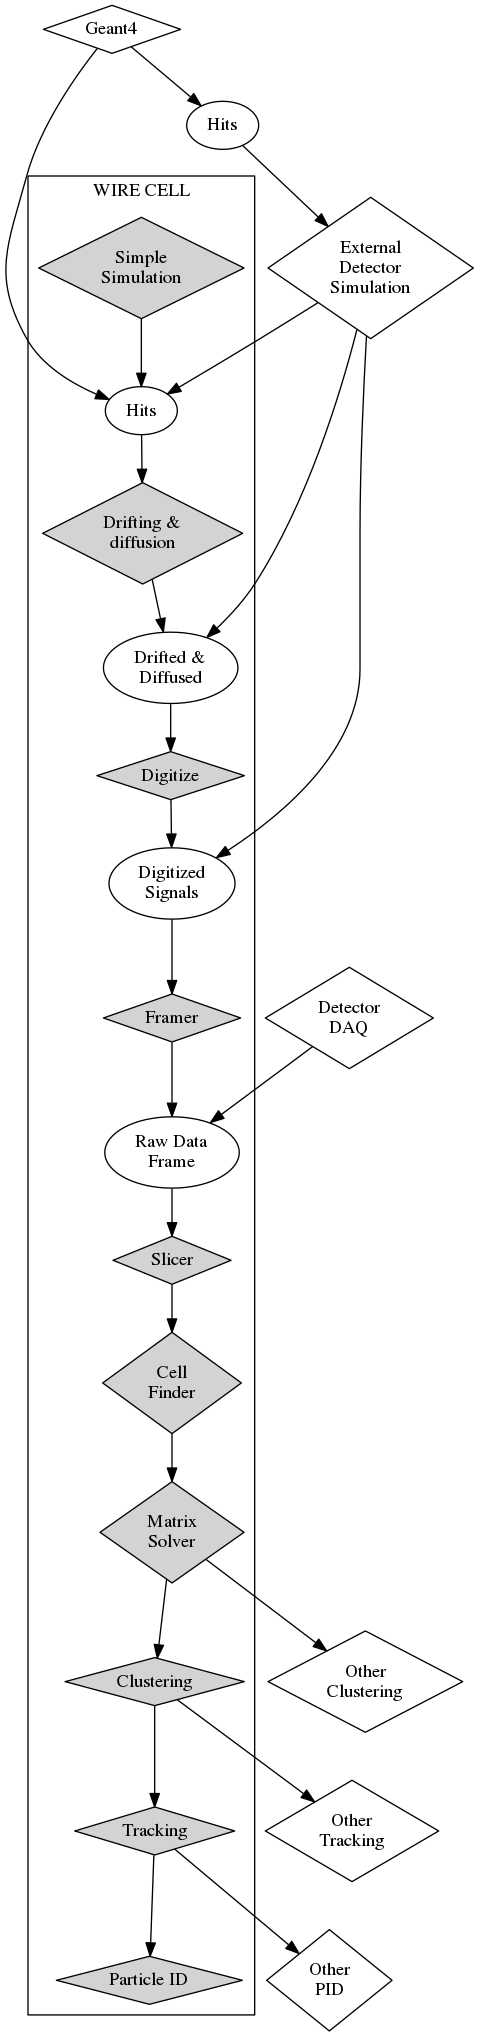
\includegraphics[height=0.8\textheight]{wirecell-dataflow-conceptual.png}
	\caption{Components of Wirecell Reconstruction Software}
	\label{fig:wirecell-diagram}
\end{figure}
Full description of Wire Cell is  beyond the scope and size limitations of this document,
so presented below is annotations for those elements of the data flow (see the diagram for specific
names) which are significant and/or present most computational challenges.

\begin{description}
\item[Slicer:] takes one "time frame" or a "readout" of raw data from DAQ (or simulated source)
and separates it in time bins.  Each bin contains ADC values for all the channels
(i.e. wires) with signal above a certain threshold that span the time bin.
	
\item[Cell Finder:] takes as a time bin and identifies ``cells'' (groups of adjacent tiles).
	
\item[Optimization Solver (aka Matrix Solver):] optimizes the likelihood of the charge contained in contiguous groups of cells
with respect to producing the observed signals on wires, utilizing a model where this relationship is expressed as a matrix.
	
\item[Clustering:] aggregates groups of cells over multiple time bins, thus creating 3D objects (``clusters'').
	
\item[Tracking:] connects clusters according to certain geometry rules, forming track candidates
	
\item[PID:] determines the type of particle based on ionization pattern, as defined by
charge depositions along the particle trajectory
	
\end{description}

Elements listed above are computationally complex for a number of different reasons. For example,
the \textit{Cell Finder} performs a search on an array of tiles and given the large number
of those may face a combinatorial challenge. The \textit{Matrix Solver} has to solve an optimization
problem involving a sparse matrix. The \textit{Tracking} component has again to find relations
between multiple pieces of data based on applications of certain rules.



\newpage